\todo{Explain the used metrics and how they relate to hypothesis}
\todo{Explain the datasets and how they differ, why they are important?}
\todo{Introduce the baselines, explain how they relate to the hypothesis, why they - are chosen, how they differ}
\todo{Explain methodology, why the chosen metric really captures the problem at - hand}
\todo{Work out differences of graph types, find similarities across datasets}
\todo{Provide the questions that are relevant for the hypothesis}
\todo{Answer these questions through metrics/results}

\refsubsection{Experiments}{subsec:experiments}
\todo{Test the hypothesis}
\todo{Tables with results}
\todo{Mention difficulties and possible solutions}
\todo{Add runtime analysis}

\paragraph{Baselines}
\paragraph{Approach}


\refsubsection{Datasets}{subsec:datasets}
\todo{Statistics about datasets and derived graphs}
\todo{Skewed classes}
\todo{Graph statistics}

\begin{figure}
\centering
\begin{tabular}{lrr}

dataset &  \# classes &  \# documents \\
\midrule
ling-spam       &  2 &  2893 \\
ng20            &  20 &  18846 \\
r8              &  8 &  9459 \\
reuters-21578   &  90 &  13328 \\
review\_polarity &  2 &  2000 \\
rotten\_imdb     &  2 &  10000 \\
tagmynews       &  7 &  32600 \\
webkb           &  7 &  8274 \\

\end{tabular}

\caption{Datasets}
\end{figure}

\refsubsection{Methods}{subsec:methods}
\todo{Pre-Processing}
\todo{CV}
\todo{Significance tests}
\todo{Combined}
\todo{Scaler}
\todo{Merging nodes?}

\refsubsection{Results and Observations}{subsec:results_and_observations}
\todo{Observations + possible explanations}
\todo{How does the results relate to hypothesis?}
\todo{Error analysis}

\paragraph{Structure Of The Used Graphs}
The co-occurrence graphs have a relatively simple structure.
Co-occurrence graphs are always connected, ie. the number of connected components is 1 (or 0 in case of an empty graph).
When the window size is 1, the graph is similar to a path, meaning that most of the nodes have a degree $< 2$. With increasing window size, the graph gets more connected.

\begin{figure}[h]
\centering
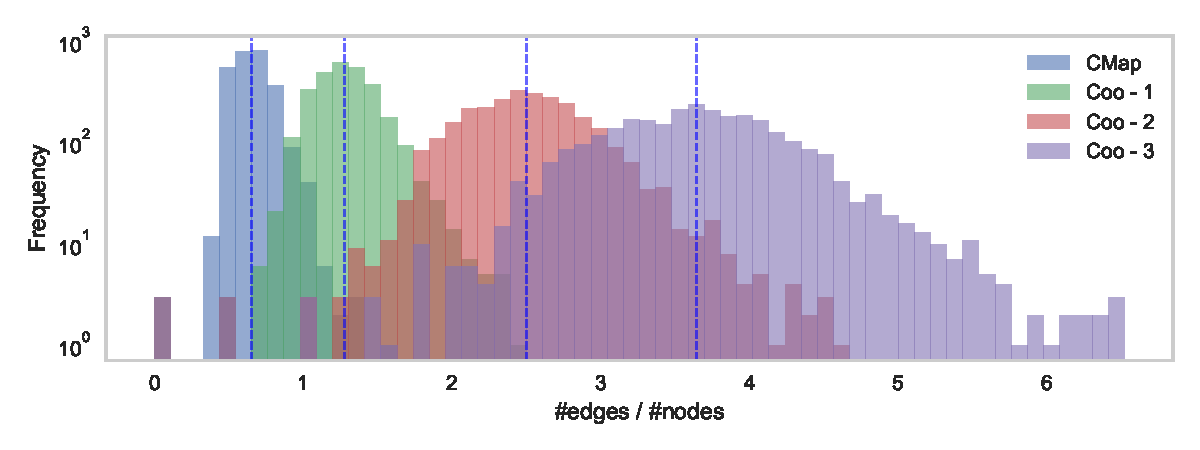
\includegraphics[width=0.7\linewidth]{assets/figures/hist-edgesnodes.pdf}
\caption{Histogram of the number of edges divided by the number of nodes. Per graph type. The lines correspond to the median value.}
\label{fig:histogram-edges-div-nodes-per-type}
\end{figure}

\begin{figure}[h]
\centering
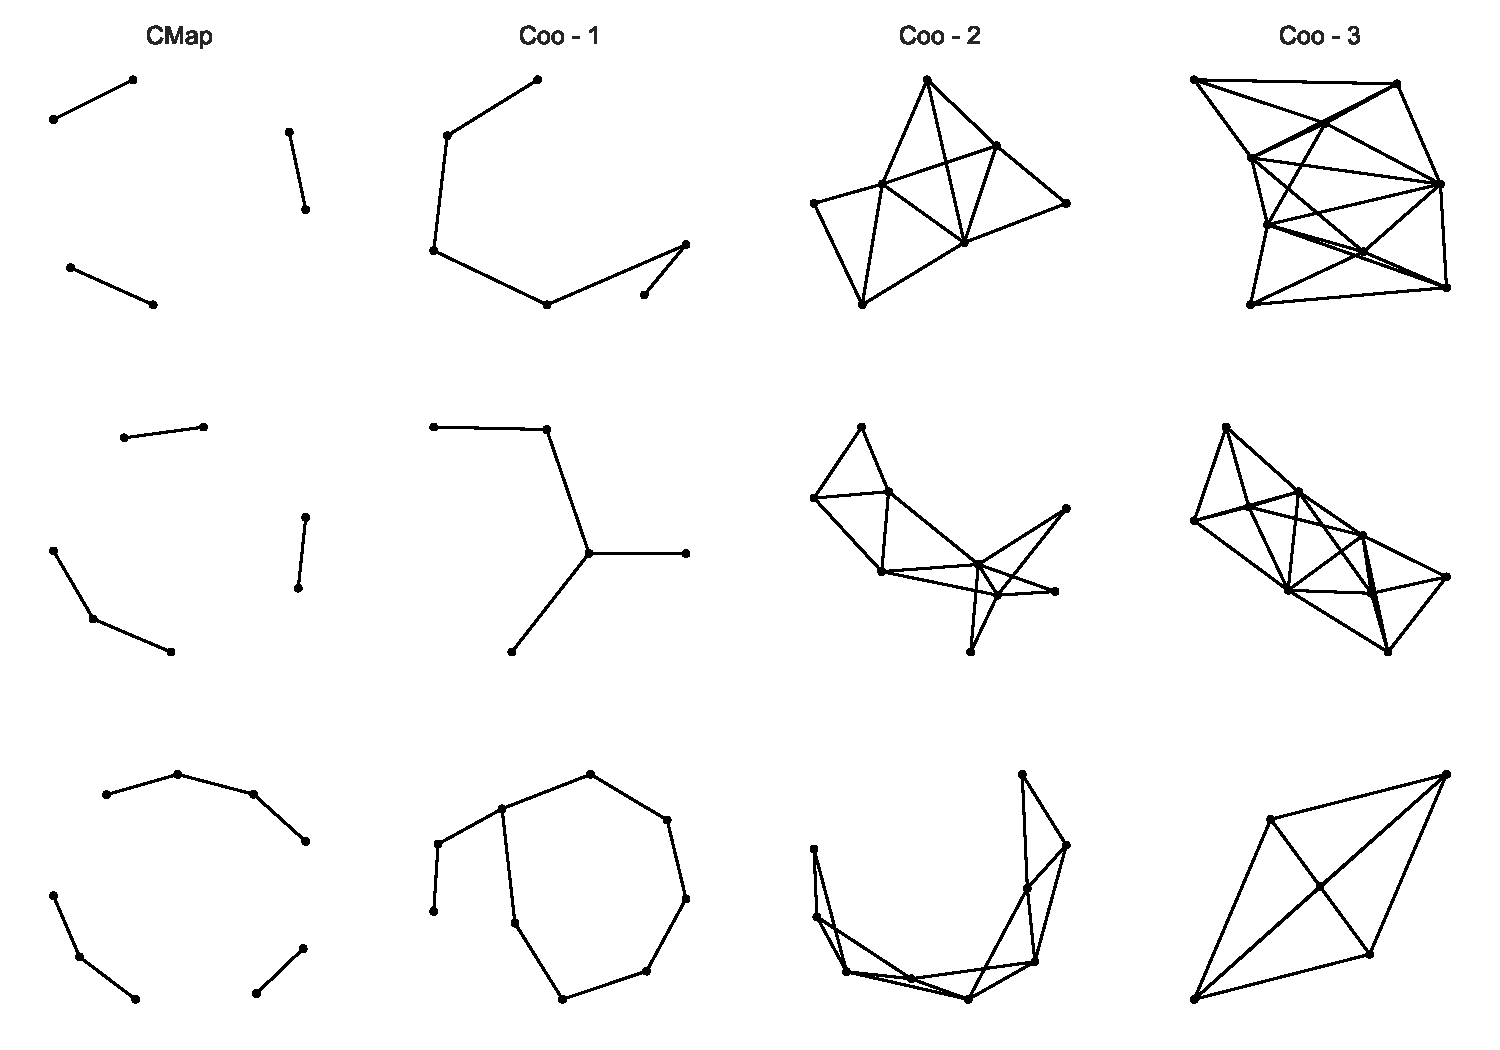
\includegraphics[width=0.6\linewidth]{assets/figures/graph-examples.pdf}
\caption{Graph examples per type. Three examples are shown per type. The concept map examples all have more than one connected component, while the co-occurrence graphs all have only one. Dataset: ling-spam}
\end{figure}

\begin{figure}[h]
\centering
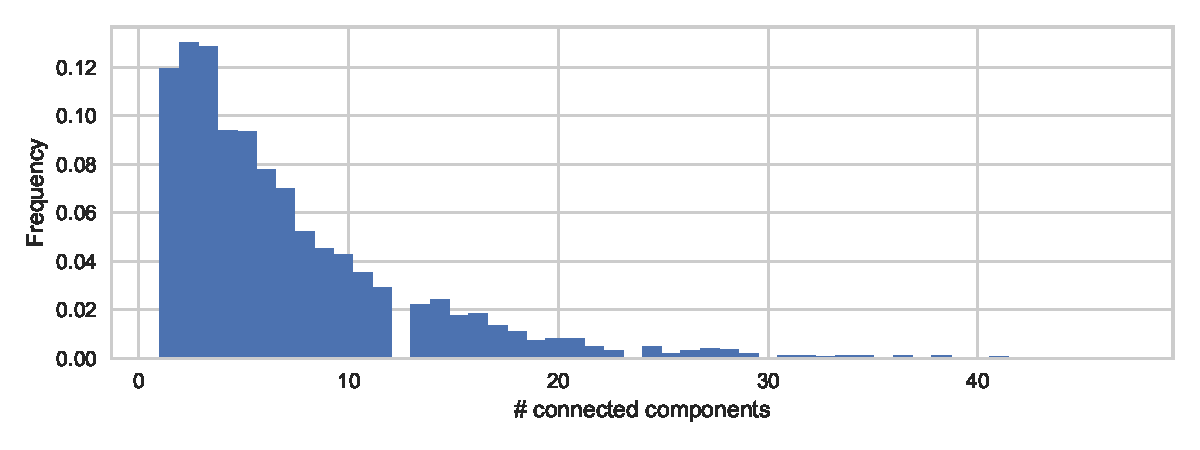
\includegraphics[width=0.8\linewidth]{assets/figures/hist-connected-components-ling-spam-CMap.pdf}
\caption{Histogram of connected components per concept map. Dataset: ling-spam.}
\end{figure}


\refsubsection{Related And Intermediate Observations}{subsec:related_and_intermediate_observation}
\todo{Sparsity of feature vectors}